\mychapter{1}{Assignment 4 \\ \vspace{-0.3cm} Explore Data and Create Linear
Regression Model}
\addcontentsline{toc}{chapter}{Assignment 4 Explore Data and Create Linear
Regression Model}
\usepackage{graphicx}

\section*{Problem Statement}
\large
Implement the following computations using Pandas and TensorFlow:

\begin{enumerate}
    \item Load the dataset and import it into a Pandas DataFrame.
    \item Display the first five rows and the last three rows of the dataset.
      \item Get the dimensions (number of rows and columns) of the dataset.
    \item Generate descriptive statistics (mean, median, standard deviation, five-point summary, IQR, etc.) for the data.
    \item Print a concise summary of the dataset as information on data types (schema) and missing values.
    \item Add a new column named “X22” by converting the “house age” from years to days.
    \item Delete the column “X22” from the dataset.
    \item Create three new instances synthetically and add them to the dataset.
    \item Delete the newly inserted three instances from the dataset.
    \item Update the “house price of unit area” to 110, provided it is currently greater than the amount.
    \item Find the latitude and longitude of the houses whose prices are less than or equal to 20.
    \item Add the missing convenience store values of instances by calculating the average number of convenience stores.
    \item Find the normalized distance to the nearest train station by performing:
    \begin{enumerate}
        \item Z-score normalization.
        \item Min-max normalization.
        \item Decimal scaling.
    \end{enumerate}
    \item Generate the following basic visualizations using Seaborn. Customize your visualizations by adding titles, labels, legends, and appropriate color schemes.
    \begin{enumerate}
        \item Create a histogram for the ‘’Y house price of unit area” attribute.
        \item Create a box-and-whisker plot for the ‘’Y house price of unit area” attribute.
        \item  Create a scatter plot showing house prices against house age.
        \item Add a second scatter plot showing house prices against distance to the nearest MRT station.
    \end{enumerate}
    \item Form the Design Matrix X of shape m × n + 1 in order to apply normal equation
method where m is the number of training examples and n is the number of input
features. Only use the two normalized input features ’X2 house age’ and ’X3 distance to the nearest MRT station’ from the dataset as second and third columns respectively and all 1 s as the first column. Also, form output vector Y of shape m × 1.
   \item Find the parameter vector \( W \) using the normal equation method as \( W = (X^T X)^{-1} X^T Y \).
    \item Implement the gradient descent algorithm with the following steps:
    \begin{itemize}
    \item Form the Design Matrix \( X \) of shape \( n \times m \). Only use the two normalized input features \textit{X2 house age} and \textit{X3 distance to the nearest MRT station} and the output vector \( Y \) of shape \( 1 \times m \).
    \item Initialize the parameter vector \( W \) of shape \( 1 \times n \) and bias \( b \) (scalar).
    \item Repeat the following steps for a certain number of iterations with learning rate \( \alpha = 0.01 \), and print the final parameter values:
    \begin{itemize}
        \item[(a)] Calculate the prediction \( \hat{Y} = WX + b \).
        \item[(b)] Compute the loss \( L = \frac{1}{2} \times (\hat{Y} - Y)^2 \).
        \item[(c)] Compute the error \( E = \hat{Y} - Y \).
        \item[(d)] Compute the gradient with respect to \( W \) as \( dW = \frac{1}{m} E \cdot X^T \) and with respect to \( b \) as \( db = \frac{1}{m} \times E \) (sum over the columns).
        \item[(e)] Update \( W = W - \alpha dW \) and \( b = b - \alpha db \).
    \end{itemize}
    \item Use TensorFlow's GradientTape() to automatically calculate the gradients in step (d) and redo the training steps to print the final parameter values.
\end{itemize}


  \item Define a class to create a Linear Regression model with methods fit and predict. Use the above iterative process to implement the model’s training within the fit method.
\end{enumerate}
\newpage

\vspace{-.15cm}
\section{Loading the Dataset}
\vspace{-.75cm}
\begin{code}
\begin{lstlisting}
 import pandas as pd
 df=pd.read_csv("Real estate-Realestate.csv")
\end{lstlisting}
\end{code}
\vspace{-1cm}
\begin{verbatim} 
\end{verbatim}
\vspace{-.6cm}
\section{Preview of DataFrame}
\vspace{-.75cm}
\begin{code}
\begin{lstlisting}
 print(df.head())
 print(df.tail(3))
\end{lstlisting}
\end{code}
\vspace{-1cm}
\begin{verbatim}
 X1 transaction date  X2 house age  X3 distance to the nearest MRT station \
 0  2012.917             32.0                               84.87882
 1  2012.917             19.5                               306.59470
 2  2013.583             13.3                               561.98450
 3  2013.500             13.3                               561.98450
 4  2012.833             5.0                                390.56840
 
    X4 number of convenience stores  X5 latitude  X6 longitude \
 0  10.0                             24.98298         121.54024
 1  9.0                              24.98034         121.53951
 2  5.0                              24.98746         121.54391
 3  5.0                              24.98746         121.54391
 4  5.0                              24.97937         121.54245
 
   Y house price of unit area
 0  37.9
 1  42.2
 2  47.3
 3  54.8
 4  43.1
 
    X1 transaction date   X2 house age \
412   2013.000                      8.1
413   2013.500                      6.5
414   2013.167                      1.9

   X3 distance to the nearest MRT station  X4 number of convenience stores \
412    104.81010                    5.0
413    90.45606                     9.0
414     355.00000                   NaN

    X5 latitude  X6 longitude Y house price of unit area
412     24.96674    121.54067                  52.5
413     24.97433    121.54310                  63.9
414     24.97293    121.54026                  40.5
\end{verbatim}

\vspace{-.75cm}
\section{Dimensions of Dataset}
\vspace{-.75cm}
\begin{code}
\begin{lstlisting}
 print(df.shape)
\end{lstlisting}
\end{code}
\vspace{-1cm}
\begin{verbatim}
 (415,7)
\end{verbatim}
\vspace{-.75cm}
\section{Descriptive Statistics}
\vspace{-.6cm}
\begin{code}
\begin{lstlisting}
 des_stat=df.describe()
 print("\nDescriptive Statistics:")
 print(des_stat)
\end{lstlisting}
\end{code}
\vspace{-.75cm}
\begin{verbatim}
 Descriptive Statistics:
        X1 transaction date   X2 house age \
count         415.000000         415.000000
mean          2013.149014        17.674458
std           0.281628           11.405161
min           2012.667000        0.000000
25%           2012.917000        8.950000
50%           2013.167000        16.100000
75%           2013.417000        28.100000
max           2013.583000        43.800000

        X3 distance to the nearest MRT station \
count                   415.000000
mean                    1082.129338
std                     1261.092057
min                     23.382840
25%                     289.324800
50%                     492.231300
75%                     1452.760000
max                     6488.021000

         X4 number of convenience stores  X5 latitude  X6 longitude \
count        414.000000                     415.000000      415.000000
mean         4.094203                       24.969039       121.533378
std          2.945562                       0.012397        0.015332
min          0.000000                       24.932070       121.473530
25%          1.000000                       24.963010       121.528570
50%          4.000000                       24.971100       121.538630
75%          6.000000                       24.977450       121.543300
max          10.000000                      25.014590       121.566270

    Y house price of unit area
count            415.000000
mean             37.986265
std              13.590608
min              7.600000
25%              27.700000
50%              38.500000  
75%              46.600000
max              117.500000
\end{verbatim}
\vspace{-.75cm}
\section{Data types and Missing values}
\vspace{-.6cm}
\begin{code}
\begin{lstlisting}
 print("\nDatasetsummary: ")
 df.info()
\end{lstlisting}
\end{code}
\vspace{-1cm}
\begin{verbatim}
 Datasetsummary:
 <class 'pandas.core.frame.DataFrame'>
 RangeIndex :415 entries, 0 to 414
 Data columns (total 7 columns):
 #    Column                                   Non-NullCount   Dtype
 ---  -------                                  -------------   ----
 0    X1 transaction date                        415non-null   float64
 1    X2 house age                               415non-null   float64
 2    X3 distance to the nearest MRT station     415non-null   float64
 3    X4 number of convenience stores            414non-null   float64
 4    X5 latitude                                415non-null   float64
 5    X6 longitude                               415non-null   float64
 6    Y house price of unit area                 415non-null   float64
 dtypes: float64(7)
 memory usage: 22.8KB
\end{verbatim}
%\vspace{-.6cm}
%\newpage
\section{Adding new column}
\begin{lstlisting}
df['X22']= df['X2houseage']* 365
 print("\n Added'x22' column:")
 print(df.head())

\end{lstlisting}
\begin{verbatim}
 Added 'x22' column:
    X1 transaction date  X2 house age  X3 distance to the nearest MRT station \
 0      2012.917            32.0                    84.87882
 1      2012.917            19.5                    306.59470
 2      2013.583            13.3                    561.98450
 3      2013.500            13.3                    561.98450
 4      2012.833            5.0                     390.56840
 
    X4  number  of convenience  stores  X5  latitude    X6  longitude \
 0      10.0                                24.98298        121.54024
 1      9.0                                 24.98034        121.53951
 2      5.0                                 24.98746        121.54391
 3      5.0                                 24.98746        121.54391
 4      5.0                                 24.97937        121.54245
 
    Y house price of unit area          X22
 0          37.9                        11680.0
 1          42.2                        7117.5
 2          47.3                        4854.5
 3          54.8                        4854.5
 4          43.1                        1825.0

\end{verbatim}
\section{Deleting column}
\begin{lstlisting}
df=df.drop(columns=['X22'])
 print("\n Deleted'X22' column:")
 print(df.head())
\end{lstlisting}
\newpage
\begin{verbatim}
Deleted 'X22' column:
     X1 transaction date  X2 house age  X3 distance to the nearest MRT station \
 0      2012.917            32.0                    84.87882
 1      2012.917            19.5                    306.59470
 2      2013.583            13.3                    561.98450
 3      2013.500            13.3                    561.98450
 4      2012.833            5.0                     390.56840
 
    X4  number  of convenience  stores  X5  latitude    X6  longitude \
 0      10.0                                24.98298        121.54024
 1      9.0                                 24.98034        121.53951
 2      5.0                                 24.98746        121.54391
 3      5.0                                 24.98746        121.54391
 4      5.0                                 24.97937        121.54245
 
    Y house price of unit area          
 0          37.9                       
 1          42.2                        
 2          47.3                       
 3          54.8                        
 4          43.1                       

\end{verbatim}
\section{Creation of Instances}
\begin{lstlisting}
 new_instances =pd.DataFrame({'column1':[10,11, 12], 'column2' [14,15,16]})
 df =pd.concat([df, new_instances],ignore_index=True)
 print("\n Added3newinstances:")
 print(df.tail(3))
\end{lstlisting}
\begin{verbatim}
 Added 3 new instances:
        X1 transaction date      X2 houseage \
 418         NaN                        NaN
 419         NaN                        NaN
 420         NaN                        NaN
 
     X3 distance to the nearest MRT station  X4 number of convenience stores \
 418                NaN                                     NaN
 419                NaN                                     NaN
 420                NaN                                     NaN
 
     X5 latitude    X6 longitude  Y house price of unit area  column1     column2
 418    NaN             NaN                     NaN             10.0          14.0
 419    NaN             NaN                     NaN             11.0          15.0
 420    NaN             NaN                     NaN             12.0          16.0                     

\end{verbatim}
\section{Deletion of Instances}
\begin{lstlisting}
 f=df.iloc[:-3]
 print("\n Deletedthe3newlyaddedinstances:")
\end{lstlisting}
\begin{verbatim}
 Deleted the3 newlyaddedinstances:               
\end{verbatim}
\section{Column Updation}
\begin{lstlisting}
 df.loc[df['Yhouse priceofunitarea'] >110, 'Yhousepriceofunitarea'] =␣
 ↪110
 print(df.head())
\end{lstlisting}
\begin{verbatim}
     X1 transaction date  X2 house age  X3 distance to the nearest MRT station \
 0      2012.917            32.0                    84.87882
 1      2012.917            19.5                    306.59470
 2      2013.583            13.3                    561.98450
 3      2013.500            13.3                    561.98450
 4      2012.833            5.0                     390.56840
 
    X4  number  of convenience  stores  X5  latitude    X6  longitude \
 0      10.0                                24.98298        121.54024
 1      9.0                                 24.98034        121.53951
 2      5.0                                 24.98746        121.54391
 3      5.0                                 24.98746        121.54391
 4      5.0                                 24.97937        121.54245
 
    Y house price of unit area   column1      column2   
 0          37.9                   Nan           Nan 
 1          42.2                   Nan           Nan 
 2          47.3                   Nan           Nan 
 3          54.8                   Nan           Nan 
 4          43.1                   Nan           Nan   
             
\end{verbatim}
\section{Latitude and Longitude}
\begin{lstlisting}
 result =df.loc[df['Y housepriceofunitarea']<=20,['X5latitude', 'X6␣
 ↪longitude']]
 print(result)
\end{lstlisting}
\begin{verbatim}
     X5 latitude     X6 longitude
 8      24.95095        121.48458
 40     24.94155        121.50381
 41     24.94297        121.50342
 48     24.94684        121.49578
 49     24.94925        121.49542
 55     24.94968        121.53009
 73     24.94155        121.50381
 83     24.96056        121.50831
 87     24.94297        121.50342
 93     24.94920        121.53076
 113    24.96172        121.53812
 116    24.94375        121.47883
 117    24.93885        121.50383
 155    24.94155        121.50381
 156    24.94883        121.52954
 162    24.94297        121.50342
 170    24.94741        121.49628
 176    24.94867        121.49507
 180    24.94898        121.49621
 183    24.94155        121.50381
 226    24.94155        121.50381
 229    24.94890        121.53095
 231    24.94235        121.50357
 232    24.95032        121.49587
 249    24.95743        121.47516
 251    24.94960        121.53018
 255    24.95095        121.48458
 298    24.94155        121.50381
 309    24.94883        121.52954
 320    24.93885        121.50383
 329    24.93885        121.50383
 330    24.94935        121.53046
 331    24.94826        121.49587
 347    24.95719        121.47353
 384    24.94297        121.50342
 409    24.94155        121.50381             
\end{verbatim}
\section{calculation of average numbers}
\begin{lstlisting}
mean_value= df['X4numberofconveniencestores'].mean()
 df['X4numberof conveniencestores']= df['X4numberofconveniencestores'].
 ↪fillna(mean_value)
 print(df.head())
\end{lstlisting}
\begin{verbatim}
     X1 transaction date  X2 house age  X3 distance to the nearest MRT station \
 0      2012.917            32.0                        84.87882
 1      2012.917            19.5                        306.59470
 2      2013.583            13.3                        561.98450
 3      2013.500            13.3                        561.98450
 4      2012.833            5.0                         390.56840
 
    X4 number of convenience stores  X5 latitude  X6 longitude \
 0      10.0                            24.98298       121.54024
 1      9.0                             24.98034       121.53951
 2      5.0                             24.98746       121.54391
 3      5.0                             24.98746       121.54391
 4      5.0                             24.97937       121.54245
    Y house price of unit area  column1  column2  z_score_normalized
 0          37.9                   NaN     NaN         -0.794584
 1          42.2                   NaN     NaN         -0.619078
 2          47.3                   NaN     NaN         -0.416917
 3          54.8                   NaN     NaN         -0.416917
 4          43.1                   NaN     NaN         -0.552606          
\end{verbatim}
\section{Normalized Distance}
\begin{lstlisting}
 df['z_score_normalized'] =(df['X3distancetothenearestMRTstation']-␣
 ↪df['X3distance tothenearestMRTstation'].mean())/df['X3distanceto␣
 ↪thenearestMRTstation'].std()
 print(df[['X3 distancetothenearestMRTstation','z_score_normalized']].
 ↪head())
  df['min_max_normalized'] =(df['X3distancetothenearestMRTstation']-␣
 ↪df['X3distance tothenearestMRTstation'].min()) /(df['X3distanceto␣
 ↪thenearestMRTstation'].max()-df['X3distancetothenearestMRT␣
 ↪station'].min())
 print(df[['X3 distancetothenearestMRTstation','min_max_normalized']].
 ↪head())
  df['decimal_scaled'] =df['X3distancetothenearestMRTstation']/␣
 ↪10**len(str(int(df['X3distancetothenearestMRTstation'].max())))
 print(df[['X3 distancetothenearestMRTstation','decimal_scaled']].head())
\end{lstlisting}
\begin{verbatim}
     X3 distance to the nearest MRT station     z_score_normalized
 0               84.87882                           -0.794584
 1               306.59470                          -0.619078
 2               561.98450                          -0.416917
 3               561.98450                          -0.416917
 4               390.56840                          -0.552606  

   X3 distance to the nearest MRT station      min_max_normalized
 0               84.87882                            0.009513
 1               306.59470                           0.043809
 2               561.98450                           0.083315
 3               561.98450                           0.083315
 4               390.56840                           0.056799 

   X3 distance to the nearest MRT station     decimal_scaled
 0               84.87882                            0.008488
 1               306.59470                           0.030659
 2               561.98450                           0.056198
 3               561.98450                           0.056198
 4               390.56840                           0.039057  
\end{verbatim}
\section{Plotting the Histogram of House Prices}
\begin{lstlisting}
 import matplotlib.pyplot as plt
 import seabornas sns
 sns.histplot(df['Yhousepriceofunitarea'])
 plt.title('HistogramofHousePrices')
 plt.show()
  sns.boxplot(y=df['Yhousepriceofunitarea'])
 plt.title('Boxplot of HousePrices')
 plt.show()
 sns.scatterplot(x=df['X2 house age'], y=df['Y house price of unit area'])
 plt.title('House Prices vs. House Age')
 plt.show()
 sns.scatterplot(x=df['X3 distance to the nearest MRT station'], y=df['Y house␣
 ↪price of unit area'])
 plt.title('House Prices vs. Distance to MRT Station')
 plt.show()
\end{lstlisting}
\vspace{-.75cm}
\begin{figure}[h!]
    \centering
    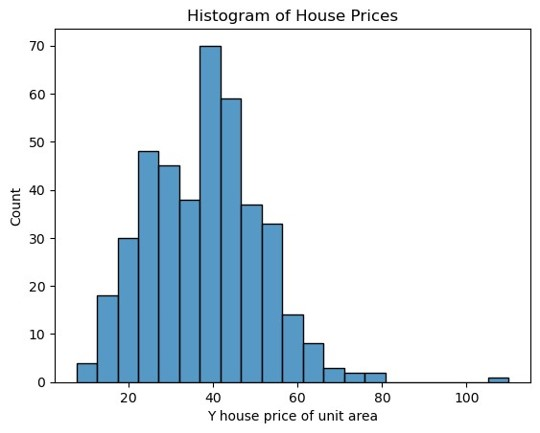
\includegraphics[width=0.8\textwidth]{histogram.png.jpg}
    \caption{Histogram of house price of unit area}
     \label{fig:histogram}
\end{figure}
\newpage
\begin{figure}[h!]
    \centering
    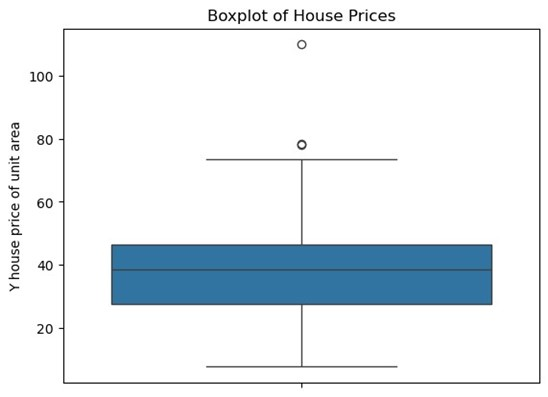
\includegraphics[width=0.8\textwidth]{boxplot.jpg}
    \caption{Histogram of house price of unit area}
     \label{fig:histogram}
\end{figure}
\vspace{-.75cm}
\begin{figure}[h!]
    \centering
    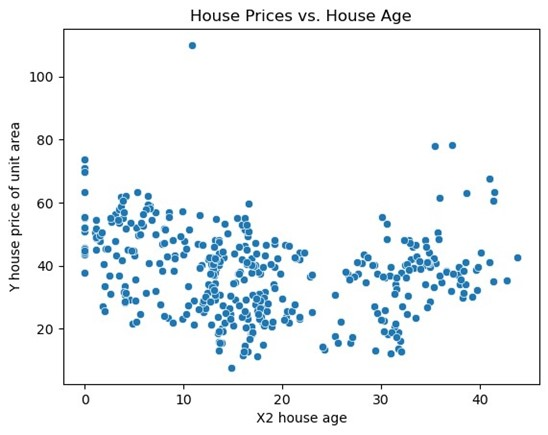
\includegraphics[width=0.8\textwidth]{scatterplot.jpg}
    \caption{Histogram of house price of unit area}
     \label{fig:histogram}
\end{figure}
\newpage
\begin{figure}[h!]
    \centering
    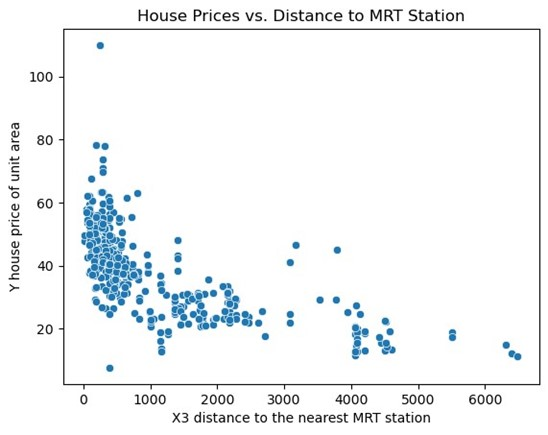
\includegraphics[width=0.8\textwidth]{scatterplot1.jpg}
    \caption{Histogram of house price of unit area}
     \label{fig:histogram}
\end{figure}
\vspace{-.75cm}
\section{Standardizing Features and Preparing Design Matrix}
\begin{code}
\begin{lstlisting}
import numpy as np
 X = np.ones((df.shape[0], 3))
 X[:, 1] = df['z_score_normalized']
 X[:, 2] = df['min_max_normalized']
 Y = df['Y house price of unit area'].values.reshape(-1, 1)
 print(X)
 print(Y)
\end{lstlisting}
\end{code}
\vspace{-.75cm}
\begin{verbatim}
  [[ 1.        -0.79458408 0.00951267] 
   [ 1.        -0.61907813 0.04380939]
   [ 1.        -0.41691656 0.08331505]
 …
 [ 1.            nan  nan]
 [ 1.            nan  nan]
 [ 1.            nan  nan]]                 
                                                            
 
 [[ 37.9]
 [ 42.2]
 [ 47.3]
 [ 54.8]
 [ 43.1]
 [ 32.1]
 [ 40.3]
 [ 46.7]
 [ 18.8]
 [ 22.1]
 [ 41.4]
 [ 58.1]
 [ 39.3]
 [ 23.8]
 [ 34.3]
 [ 50.5]
 [ 70.1]
 [ 37.4]
 [ 42.3]
 [ 47.7]
 [ 29.3]
 [ 51.6]
 [ 24.6]
 [ 47.9]
 [ 38.8]
 [ 27. ]
 [ 56.2]
 [ 33.6]
 [ 47. ]
 [ 57.1]
 [ 22.1]
 [ 25. ]
 [ 34.2]
 [ 49.3]
 [ 55.1]
 [ 27.3]
 [ 22.9]
 [ 25.3]
 [ 47.7]
 [ 46.2]
 [ 15.9]
 [ 18.2]
 [ 34.7]
 [ 34.1]
 [ 53.9]
 [ 38.3]
 [ 42. ]
 [ 61.5]
 [ 13.4]
 [ 13.2]
 [ 44.2]]
\end{verbatim}
\vspace{-.75cm}
\section{Calculating Regression Parameters Using Matrix Operations}
\begin{code}
\begin{lstlisting}
W = np.linalg.inv(X.T @ X) @ X.T @ Y
 print("Parameter Vector W (Normal Equation):", W)
\end{lstlisting}
\end{code}\begin{verbatim}
     Parameter Vector W (Normal Equation): [[nan]
 [nan]
 [nan]]
\end{verbatim}
\vspace{-.75cm}
\newpage
\section{Linear Regression with Manual Gradient Descent and TensorFlow GradientTape}
\begin{code}
\begin{lstlisting}
import numpy as np
 import tensorflow as tf
 # Example data
 X = np.random.randn(421, 2).astype(np.float32)
Y = np.random.randn(421, 1).astype(np.float32)
 # Convert to TensorFlow tensors
 X_tf = tf.convert_to_tensor(X)
 Y_tf = tf.convert_to_tensor(Y)
 # Initialize weights and bias
 W = tf.Variable(tf.random.normal((1, 2)))
 b = tf.Variable(tf.random.normal((1,)))
 # Define the loss function
 def compute_loss():
 Y_hat = tf.matmul(X_tf, W, transpose_b=True) + b
 return tf.reduce_mean(0.5 * tf.square(Y_hat- Y_tf))
 # Define the optimizer
 optimizer = tf.optimizers.SGD(learning_rate=0.01)
 # Training loop
 epochs = 1000
 for i in range(epochs):
 with tf.GradientTape() as tape:
 loss = compute_loss()
 grads = tape.gradient(loss, [W, b])
 optimizer.apply_gradients(zip(grads, [W, b]))
 print("Final Weights (TensorFlow):", W.numpy())
 print("Final Bias (TensorFlow):", b.numpy())
\end{lstlisting}
\end{code}
\begin{verbatim}
 Final Weights (TensorFlow): [[-0.01636326-0.07295796]]
 Final Bias (TensorFlow): [0.0130949]
\end{verbatim}
\section{Implementing and Using a Custom Linear Regression Class}
\begin{code}
\begin{lstlisting}
 import numpy as np
 import pandas as pd
 import tensorflow as tf
 # Create a sample DataFrame
 data = {
 'X2 house age': np.random.rand(100),
 'X3 distance to the nearest MRT station': np.random.rand(100),
 'Y house price of unit area': np.random.rand(100)
 }
 df = pd.DataFrame(data)
 # Convert DataFrame columns to TensorFlow tensors
 XT = tf.convert_to_tensor(
 df[['X2 house age', 'X3 distance to the nearest MRT station']].values,
 dtype=tf.float32
 )
 X = tf.transpose(XT) # Input matrix of shape (n, m)
 Y = tf.convert_to_tensor(
 df['Y house price of unit area'].values.reshape(1,-1),
 dtype=tf.float32
 ) # Target vector of shape (1, m)
 # Define model parameters
 m = X.shape[1] # Number of samples
 n = X.shape[0] # Number of features
 W = tf.Variable(tf.random.uniform((1, n), minval=0, maxval=1), dtype=tf.float32)
 B = tf.Variable(tf.random.uniform((1,), minval=0, maxval=1), dtype=tf.float32)
 # Training parameters
 learning_rate = 0.01
 num_iterations = 10000
 # Gradient Descent Loop
 for step in range(num_iterations):
 with tf.GradientTape() as tape:
 # Forward pass
 Y_hat = tf.matmul(W, X) + B
 error = Y_hat- Y
 loss = tf.reduce_mean(tf.square(error)) # Mean Squared Error Loss
 # Compute gradients
 grad_W, grad_B = tape.gradient(loss, [W, B])
 # Update weights and bias
 W.assign_sub(learning_rate * grad_W)
 B.assign_sub(learning_rate * grad_B)
 # Print loss and parameters at intervals
 if (step + 1) % 1000 == 0:
 print(f"Epoch {step + 1}: Loss = {loss.numpy()}, W = {W.numpy()}, B =␣
 ↪{B.numpy()}")
\end{lstlisting}
\end{code}
\begin{verbatim}
Epoch 1000: Loss = 0.08621952682733536, W = [[-0.11358874 0.10545328]], B =[0.52158034]
 Epoch 2000: Loss = 0.08483896404504776, W = [[-0.09776288 0.00779503]],
 B =[0.5688425]
 Epoch 3000: Loss = 0.08471596986055374, W = [[-0.10272954-0.01955936]],
 B =[0.5872949]
 Epoch 4000: Loss = 0.08470050990581512, W = [[-0.10686363-0.02813785]], 
 B =[0.59451085]
 Epoch 5000: Loss = 0.08469826728105545, W = [[-0.10891178-0.03107916]], 
 B =[0.597335]
 Epoch 6000: Loss = 0.08469793200492859, W = [[-0.10979746-0.03214846]], 
 B = [0.59843946]
 Epoch 7000: Loss = 0.08469788730144501, W = [[-0.11016019-0.03255066]],
 B = [0.5988717]
 Epoch 8000: Loss = 0.08469786494970322, W = [[-0.1103053-0.0327049]], B =[0.59904146]
 Epoch 9000: Loss = 0.08469786494970322, W = [[-0.11036471-0.03276638]],
 B = [0.59910977]
 Epoch 10000: Loss = 0.08469786494970322, W = [[-0.11038668-0.03278921]],
 B = [0.5991339]
\end{verbatim}



